\section{SE(2) Filter}

\subsection{Lie Gruppe}
 Eine Lie-Gruppe G ist eine Mannigfaltigkeit G, welche zusammen mit einer glatten Operation 
 
 \begin{equation*}
  G\times G\ni (g_{1},g_{2})\to g_{1}\cdot g_{2}\in G
 \end{equation*}
eine Gruppe ist.


Ein Vorteil der abstrakten Definition von Lie-Gruppe besteht darin, dass sie wesentlich flexibler ist. Zum Beispiel gilt folgendes: Ist G eine Lie-Gruppe und N ein abgeschlossener Normalteiler, dann ist G/N wieder eine Lie-Gruppe.


\subsection{SE(2)-Bingham-Verteilung}
In diesem Projekt verwenden wir einen Filter, der auf der SE(2)-Bingham-Verteilung für zweidimensionale Translationensvektoren und einem Skalar für die Rotation basiert. Die SE(2)-Bingham-Verteilung kann zur Darstellung der Orientierungen auf der Ebene verwendet werden. [5]
Anstatt sich auf die auf Gauß'sche-Verteilung basierende Annäherungen zu verlassen, haben wir uns entschieden, alle auftretenden Wahrscheinlichkeiten durch SE(2)-Bingham-Verteilung darzustellen. Diese verwendet für die Translation weiterhin eine zweidimensionale Normalverteilung, kombiniert mit einer Bingham-Verteilung, die auf der Hypersphere der Rotationen definiert wird. Die  antipodisch Symmetrie ist in Abbildung \ref{fig:bingham} gezeigt.

\begin{figure}
	\centering
	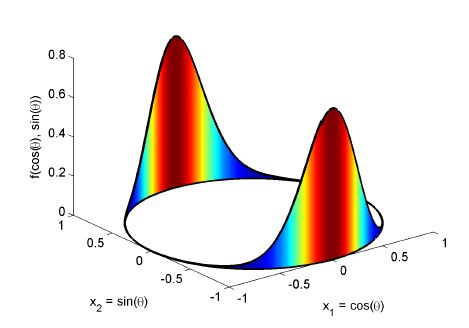
\includegraphics[width=0.7\linewidth]{Images/bingham}
	\caption{Darstellung von hypersphärischen Zufallsvektoren [2] }
	\label{fig:bingham}
\end{figure}

In unsere Fall ist die Bingham-Verteilung einfacher für die Darstellung der Orientierung des Laufroboters. Als eine Folge der obigen Motivation kann man sehen, dass die Bingham- Wahrscheinlichkeits- dichtefunktion (pdf) zwei symmetrische Moden aufweist. Die Parametermatrix der Bingham-Verteilung aus der Exponentialfunktion  (welche die inverse  Kovarianzmatrix im Gauß'schen Fall ist) wird üblicherweise zerlegt in eine orthogonale und eine diagonale Matrix. Dies führt zu der folgenden Definition:
\begin{equation}
	f\left(\vec{x}\right)=\frac{1}{F}\cdot exp\left(\vec{x}^{T}MZM^{T}\vec{x}\right)
\end{equation}




\subsection{Duale Quaternionen}
In unsere Projekt werden duale Quaternionen zur Darstellung der Starrkörperbewegung verwendet. Die dualen Quaternionen werden durch folgende Formel darstellt [1]

\begin{equation}
\sigma=p+\epsilon q
\end{equation}
Unter Ihnen die p steht für jeweilige Quaternionen
\begin{equation}
	p=p_{0}+\vec{p}=p_{0}+p_{1}\vec{i}+p_{2}\vec{j}+p_{3}\vec{k}
\end{equation}
\begin{equation}
	q=q_{0}+\vec{q}=q_{0}+q_{1}\vec{i}+q_{2}\vec{j}+q_{3}\vec{k}
\end{equation}
Für die duale Einheit $\epsilon$ gitl $\epsilon^2 = 0$.

Die Rotationsmatrix R, Translationsvektor t kann kompakt durch eine duales Quaternion dargestellt werden. Der Translationsvektor t ist ein reines Quaternion. Wir kombinieren es mit dem Rotationsquaternion $r =\cos\frac{\theta}{2}+ \vec{\widehat{u}}sin\frac{\theta}{2}$, das die Rotation um den Vektor $\widehat{u}$ beschreibt, zu dem folgendem dualem Quaternion:

\begin{equation}
	\sigma = r + \frac{\epsilon}{2}\vec{t}r\\
	=cos\frac{\theta}{2}+ \vec{\widehat{u}}sin\frac{\theta}{2} + \frac{\epsilon}{2}\left( -sin\frac{\theta}{2}\left(\vec{t}\cdot\widehat{u} \right)+ cos\frac{\theta}{2} \vec{t}+sin\frac{\theta}{2} \vec{t} \times \widehat{u} \right) 
\end{equation}

In unseren Fall wird die Bewegung der Roboter hauptsächlich auf eine Eben durchgeführt werden. Deshalb stehen $\vec{t}_{x}$ und $\vec{t}_{y}$ für die Translation des Roboters und $\theta$ für die Rotation. Um Rotationen und Translationen in 2D zu kombinieren, wird hier
duale Quaternion-Multiplikation verwendet. Eine Rotation mit anschliesender Translation wird durch die Multiplikation beschrieben.
\begin{equation}
	\left[1+\epsilon\frac{1}{2}\left(t_{x}\vec{i}+t_{y}\vec{j}\right) \right] \cdot\left[cos\left( \frac{\alpha}{2}\right)+sin\left(\frac{\alpha}{2}\right)\vec{k}\right]
\end{equation}
